%Document-Author: Davide Tommasin
%Document-Date: 2016/05/12
%Document-Description: Manuale Utente del gruppo SWEeneyThreads 

\documentclass[a4paper]{article}
\usepackage[english, italian]{babel}
\usepackage[T1]{fontenc}
\usepackage[utf8]{inputenc}
\usepackage{url}
\usepackage{graphicx}
\usepackage[hidelinks]{hyperref}
\usepackage{booktabs}
\usepackage{eurosym}
\usepackage{tabularx}
\usepackage{pifont}
\usepackage[table]{xcolor}
\usepackage{float}
\usepackage[]{appendix}
\usepackage{ltxtable} 
\usepackage{geometry}
\geometry{margin=1in}
\usepackage{longtable}
\usepackage{multirow}

\graphicspath{{Immagini/}}

\newcolumntype{Y}{>{\centering\arraybackslash}X}
\newcolumntype{s}{>{\hsize=.21\hsize}X}
\newcolumntype{f}{>{\hsize=.37\hsize}X}
\newcolumntype{m}{>{\hsize=.42\hsize}X}
\newcolumntype{t}{>{\hsize=.1\hsize}X}
\newcolumntype{r}{>{\hsize=.3\hsize}X}
\newcolumntype{k}{>{\hsize=.4\hsize}X}

\renewcommand{\abstractname}{Tabella contenuti}

\begin{document}
	
	\begin{titlepage}
		% Defines a new command for the horizontal lines, change thickness here
		\newcommand{\HRule}{\rule{\linewidth}{0.5mm}} 
		\center  
		
		% HEADING SECTION
		\textsc{\LARGE SWEeneyThreads}\\[1.5cm] 
		\textsc{\Large Actorbase}\\[0.5cm] 
		\textsc{\large a NoSQL DB based on the Actor model}\\[0.5cm]
		
		
		% TITLE SECTION
		\HRule \\[0.4cm]
		{ \huge \bfseries User Manual}\\[0.4cm] 
		\HRule \\[1.5cm]
		
		% AUTHOR SECTION
		\begin{minipage}{0.4\textwidth}
			\begin{flushleft} \large
				\emph{Redattori:}\\
				Maino Elia \newline
				Bortolazzo Matteo \\
			\end{flushleft}
		\end{minipage}
		~
		\begin{minipage}{0.4\textwidth}
			\begin{flushright} \large
				\emph{Approvazione:} \\
				\emph{Verifica:} 
			\end{flushright}
		\end{minipage}
		
		%immagine
		\begin{figure}[H]
			\centering
			
\includegraphics[scale=0.8]{sweeney.png}
		\end{figure}
		\begin{center}
			Versione 1.0.2
		\end{center}
		% Date, change the \today to a set date if you want to be precise
		{\large \today}\\[3cm] 
		% Fill the rest of the page with whitespace
		\vfill  
	\end{titlepage}
	
	
	\tableofcontents
	
	\newpage
	\section*{History log}
		\LTXtable{\textwidth}{Tabelle/tabelle_diario_modifiche/tabella_manualeutenteENG.tex}	

	\newpage 
    \section{Introduction}
	\subsection{Document's purpose}
		The present document represents the user manual for the use of \emph{Actorbase}, a NoSQL database. All the user application's features will be described in detail. The manual is divided into three main sections, related to the main components of the product: Client, Server and Driver.
	\subsection{Product's purpose}
		The project's purpose is the development of a key-value NoSQL Database based on the actor model, with the goal of supply an appropriate technology for the development of modern applications which request very short response time, and which elaborate substantial amount of data. The development will lead to the release of the software under MIT license.
	\subsection{Glossary}
		In order to avoid language ambiguities and to maximize documents' comprehension, the group wrote \emph{Glossario v2.0.0}. In it will be defined, in a clear and concise way, the terms which could lead to ambiguities or text incomprehensions.
	\subsection{References}
	\subsubsection{Normative}
		\begin{itemize}
			\item \textbf{Norme di progetto:} \emph{Norme di progetto v3.0.0}
			\item \textbf{Capitolato d'appalto Actorbase (C1):} \\ 
			\url{http://www.math.unipd.it/~tullio/IS-1/2015/Progetto/C1p.pdf}
		\end{itemize}
	\newpage

	\section{Actorbase}
	\emph{Actorbase} is a key-value NoSQL database based on the actor model, which guarantees high level of scalability, resilience and performance. It allows to manage easily and flexibly your data, using the main advantages offered by the actor model, in order to support the development of modern and performing applications.
	\\ \\
	\emph{Actorbase} provides a command line client interface which offers an easy way to handle data as strings. With the CLI is possible to communicate quickly and intuitively with a server.
	\\ \\
	For more flexible queries it's avaiable the \emph{Scala} driver, integrable in every Java application.
	\begin{figure}[H]
		\centering
		
\includegraphics[scale=0.4]{actorbaseLogo.png}
		\caption{Actorbase Logo}
	\end{figure}

	\newpage



	\section{System requirements}	
	The correct execution of \emph{Actorbase} is guaranteed on machines that meet the subsequent hardware and software specifications.
	\\ \\
	OS:
	\begin{itemize}
		\item Windows 7 or newer
		\item OS X 10.7 or newer
		\item Ubuntu 14.04 or newer
	\end{itemize}
	Java Virtual Machine (JVM) 8 or newer.
	\\ \\
	RAM:
	\begin{itemize}
		\item Client application: 2GB minimum
		\item Server application: 4GB minimum, 8GB recommended
	\end{itemize}
	There aren't explicit requirements for the processor architecture or speed. Using a very old processor could slow down the system performances.

	\section{Installation}
	\emph{Actorbase} runs on JVM, that's the reason why it doesn't need an installation procedure (just click on the launch icon). 
	\newpage



	\section{Server application}
	The server application allows the user to run and manage an \emph{Actorbase} server instance on the machine. Once started, the server allows clients to connect to the machine, and to query the database.
	
	\subsection{Server configuration}
	The server machine's configuration is made by changing \texttt{server.conf} file. The configuration file allows the administrator to set the IP addresses and the connection ports
	\\
	If the user tries to run the server application without having defined the configuration parameters, the server will display an error message and won't start.
	
	\subsection{Server interface}
	Once the administrator has modified the configuration file it is possible to start the application by click on the icon. The server application provides the user a command line interface which displays the operation log in real time.
	\begin{figure}[H]
		\centering
		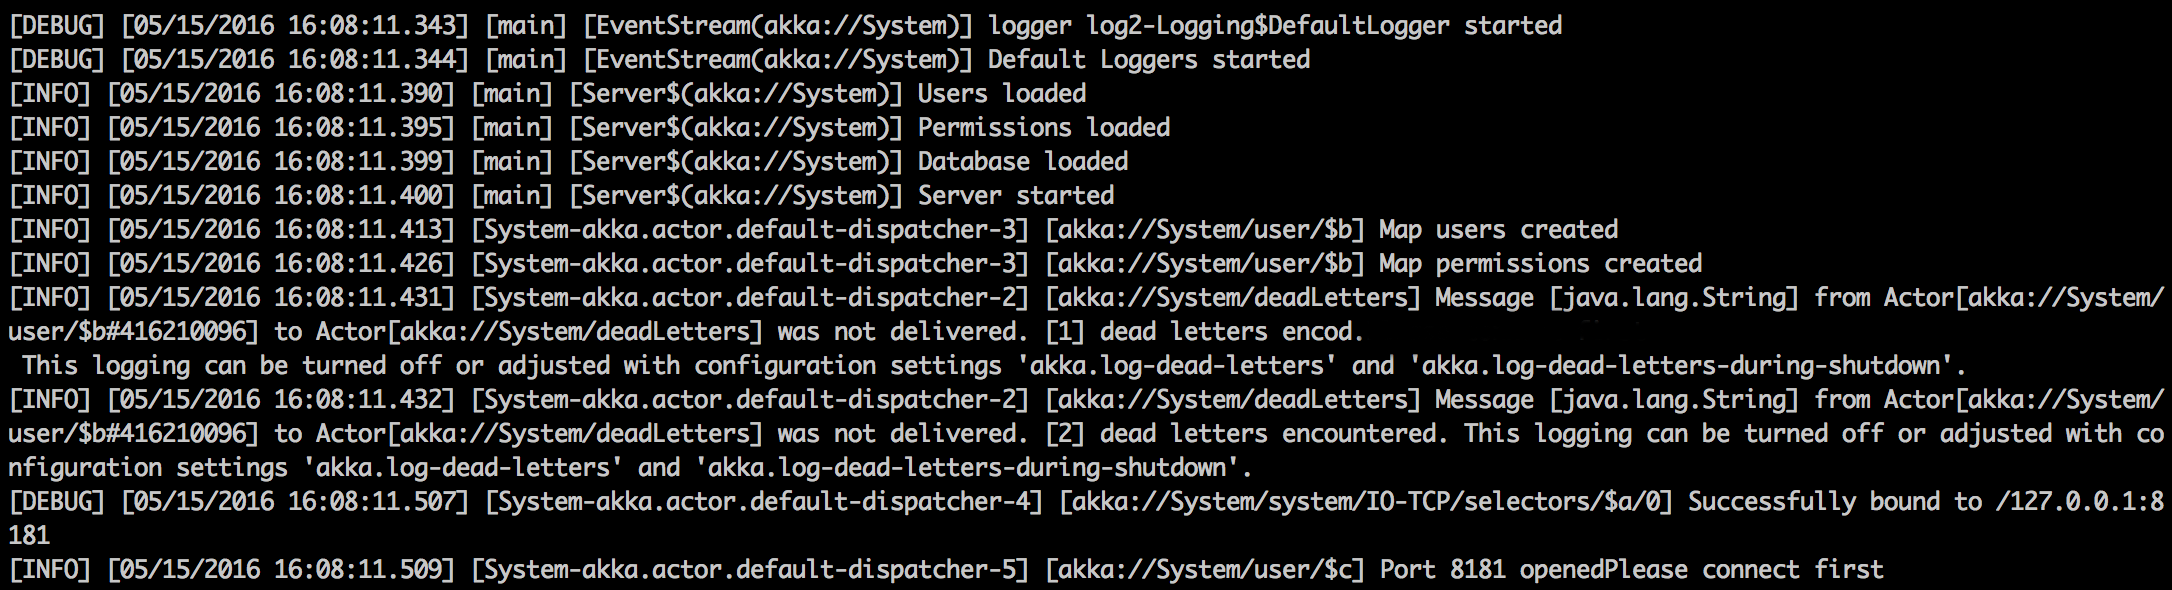
\includegraphics[width=\textwidth]{logServer.png}
		\caption{Server's log interface}
	\end{figure}
	\newpage
	

	\section{Client application}
	The client application provides a command line interface to connect to an \emph{Actorbase} server and to query it. To start the client just double-click on the client's icon. Once started, the client presents a welcome banner followed by a brief description of the software's configuration used (JVM version and operating system).
	\begin{figure}[H]
		\centering
		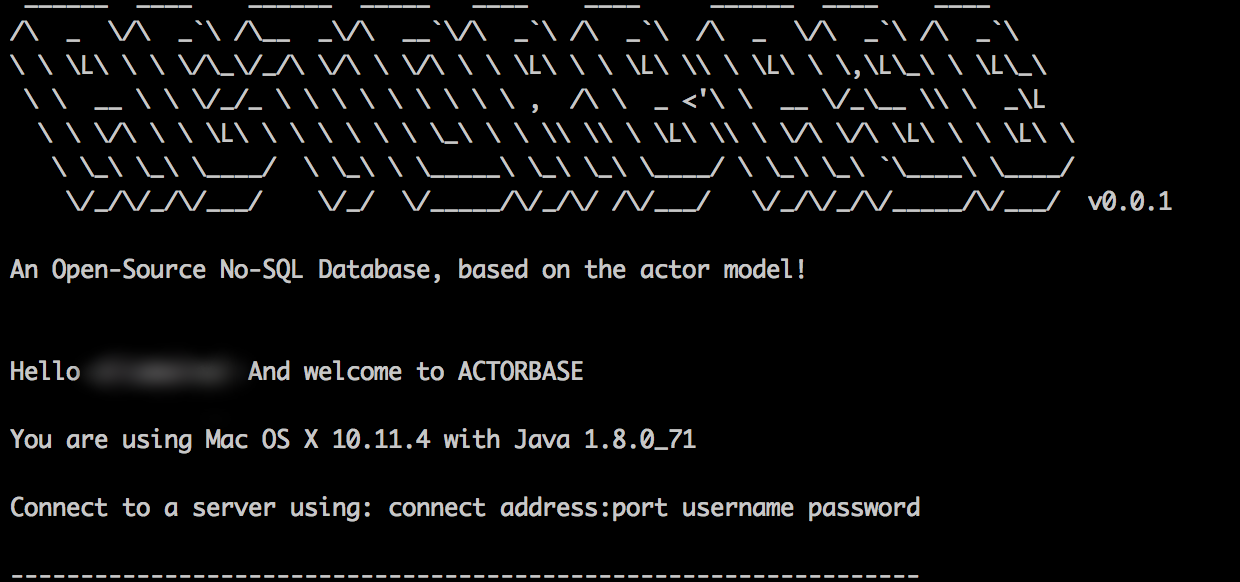
\includegraphics[width=\textwidth]{welcomeClient.png}
		\caption{Client's welcome banner}
	\end{figure}
	The interaction with the client interface is made with textual commands. They can be composed of multiple fields, separated by a space character.
	
	\subsection{Connection management}
	Once the client is running, the first thing to do is to connect to a server. The connection management is based on two commands: \texttt{connect} and \texttt{disconnect}. The application doesn't allow to manage more than one connection at time.
	
	\subsubsection{\texttt{connect} command}
	This command allows the user to connect to a server, the command structure is:
	\\ \\
	\texttt{actorbase>	connect address username password}
	\\ \\
	The server address has to be written in the format \texttt{serverAddress:port}. \\ \\
	In case of success the user receives a confirm message (\texttt{"You are connected!"}), if not, the user receives an error message (\texttt{"Connection failed!"}).
	
	\subsubsection{\texttt{disconnect} command}
	To disconnect from the server, the user just has to insert the command \texttt{disconnect} and press enter.
	
	\subsubsection{\texttt{quit} command}
	To quit the client, the user just has to insert the command \texttt{quit} and press enter.

	\subsection{Inline help}
	It is possible to obtain an help for the allowed operations, directly from the command line. The command \texttt{help} allows to obtain a generic help or a specific one.
	
	\subsubsection{Generic \texttt{help} command}
	Generic help command doesn't requests more parameters and prints on screen the \emph{Actorbase} commands list. Each command is followed by a brief description which explains his behaviour.
	
	\subsubsection{Specific \texttt{help} command}
	Specific help command has this structure:
	\\ \\
	\texttt{actorbase>	help commandName}
	\\ \\
	It allows to request informations for a particulare command, and to obtain a description of it.
	
	\subsection{Server level operations commands}
	Once connected the user is at "server level". At this level the user can do operation the following operations:
	\begin{itemize}
		\item Show the databases list
		\item Select a database
		\item Create a database
		\item Remove a database
	\end{itemize}
	
	\subsubsection{\texttt{listdb} command}
	This command allows the user to obtain, the list of databases of which the user has some access permission. The command does not request additional parameters.
	\\ \\
	\texttt{actorbase>	listdb}

	\subsubsection{\texttt{selectdb} command}
	This command allows the user to select a database. Once selected a database the user can execute operations on its maps. The command structure is the sequent:
	\\ \\
	\texttt{actorbase>	selectdb databaseName}
	\\ \\
	In case the user has the requested permissions, he receives a confirmation message: \texttt{"Database x selected"}. If not an invalid operation is reported.

	\subsubsection{\texttt{createdb} command}
	This commands allows the user to create a new database with the name specified, in case a database with that name isn't present already.
	\\ \\
	\texttt{actorbase>	createdb databaseName}
	\\ \\
	If a database with the inserted name already exists the creation fails, the user receives an error message: \texttt{"A database with the requested name already exists"}.

	\subsubsection{\texttt{deletedb} command}
	This command allows the user to delete a database from the server:
	\\ \\
	\texttt{actorbase>	deletedb databaseName}
	\\ \\
	If the user tries to remove a database than does not exist, or a database on which he does not have the modify permissions, the user receives an error message of invalid operation.
	

	\subsection{Database level operations commands}
	Once the user has selected a database with the \texttt{selectdb} command, he is at "database level". At that level a user can do these operations:
	\begin{itemize}
		\item Display the list of the maps which compose the database
		\item Map selection
		\item Map creation
		\item Map removal
	\end{itemize}

	\subsubsection{\texttt{listmap} command}
	The command show every map within the selected database.
	\\ \\
	\texttt{actorbase>	listmap}

	\subsubsection{\texttt{selectmap} command}
	This command allows to select a map using the following sintax:
	\\ \\
	\texttt{actorbase>	selectmap nomeMappa}
	\\ \\
	If the selection is confirmed the message \texttt{"Map x selected"} is showed, otherwise an \texttt{"Invalid operation"} message is showed.

	\subsubsection{\texttt{createmap} command}
	This command allows to create a map with the specified name within the selected database.
	\\ \\
	\texttt{actorbase>	createmap nomeMappa}
	\\ \\
	If the creation is confirmed the message \texttt{"Map x created"} is showed, otherwise an \texttt{"Invalid operation"} message is showed if the user doesn't have write permissions on the database or if a map with that name already exists.
	
	\subsubsection{\texttt{deletemap} command}
	This command allows to delete  a map within the selected database.
	\\ \\
	\texttt{actorbase>	deletemap nomeMappa}
	\\ \\
	If the delete is confirmed the message \texttt{"Map x deleted"} is showed, otherwise an \texttt{"Invalid operation"} message is showed if the user doesn't have write permissions on the database or if a map with that name doesn't exists.
	

	\subsection{Map level operations commands}
	Once selected a map via the command \texttt{selectmap}, the user is at the "map level". At this level the following operations are allowed:
	\begin{itemize}
		\item Show the list of keys in a map
		\item Find an item's value
		\item Insert an item
		\item Update an item's value
		\item Remove an item
	\end{itemize}

	\subsubsection{\texttt{keys} command}
	This command shows the list of all keys within the selected map
	\\ \\
	\texttt{actorbase>	keys}

	\subsubsection{\texttt{find} command}
	This command allows to get the value of an item in the map searching by his key.
	\\ \\
	\texttt{actorbase>	find key}
	\\ \\
	If the map contains an item with the inserted key the client shows the value of the item otherwise an error is showed.
	\subsubsection{\texttt{remove} command}
	This command allows to remove an item within the map:
	\\ \\
	\texttt{actorbase>	remove key}
	\\ \\
	If the remove is confirmed the message \texttt{"Item removed"} is showed, otherwise an \texttt{"No item with this key"} message is showed.

	\subsubsection{\texttt{insert} command}
	This command allows to insert an item (key-value) within the map:
	\\ \\
	\texttt{actorbase>	insert key value}
	\\ \\
	If the insert is confirmed the message \texttt{"Item inserted"} is showed, otherwise an \texttt{"An item with this key already exists"} message is showed.
	
	\subsubsection{\texttt{update} command}
	This command allows to update an item's value within the map:
	\\ \\
	\texttt{actorbase>	update key value}
	\\ \\
	If the update is confirmed the message \texttt{"Item updated"} is showed, otherwise an \texttt{"No item with this key"} message is showed.
	
	\subsection{Administrator operations commands}
	A user logged as admin can do the following operations:
	\begin{itemize}
		\item User list
		\item Add an user
		\item Remove an user
		\item User's permissions list
		\item Add/update a database permission to an user
		\item Remove a database permission to an user
		\item Set the max number of rows per Storekeeper
		\item Set the number of Ninja per Storekeeper
		\item Set the number of Warehouseman per Storekeeper
		\item Set the max number of Storekeeper per Storefinder
		\item Set the max number of Storefinder per Storemanager
	\end{itemize}

	\subsubsection{\texttt{listuser} command}
	The command shows every user on the database.
	\\ \\
	\texttt{actorbase>	listmap}

	\subsubsection{\texttt{adduser} command}
	This command allows to add an user:
	\\ \\
	\texttt{actorbase>	adduser username password}
	\\ \\
	If the add is confirmed the message \texttt{"User x added"} is showed, otherwise an \texttt{"User already exists"} message is showed if an user with that username already exists.

	\subsubsection{\texttt{removeuser} command}
	This command allows to remove an user:
	\\ \\
	\texttt{actorbase>	removeuser username}
	\\ \\
	If the remove is confirmed the message \texttt{"User x removed"} is showed, otherwise an \texttt{"User doesn't exists"} message is showed if an user with that username doesn't exists exists.
	
	\subsubsection{\texttt{listpermission} command}
	The command shows every user's permissions on the database.
	\\ \\
	\texttt{actorbase> listpermission}

	\subsubsection{\texttt{addpermission} command}
	This command allows to add a database permission to an user:
	\\ \\
	\texttt{actorbase>	addpermission username database permissionType}
	\\ \\
	If the add is confirmed the message \texttt{"Permission x added to user"} is showed, otherwise an \texttt{"User doesn't exists"} message is showed if an user with that username doesn't exists or \texttt{"Database doesn't exists"} a database with that name doesn't exists.

	\subsubsection{\texttt{removepermission} command}
	This command allows to remove a database permission to an user:
	\\ \\
	\texttt{actorbase>	removepermission username database}
	\\ \\
	If the remove is confirmed the message \texttt{"Permission x remove to user"} is showed, otherwise an \texttt{"A permission for that database doen't exists"} message is showed if a permission for that database of that user doesn't exits.
	
	\subsubsection{\texttt{setmaxrows} command}
	This command allows to set the max number of rows for each Storekeeper:
	\\ \\
	\texttt{actorbase>	setmaxrows number}

	\subsubsection{\texttt{setninja} command}
	This command allows to set the number of Ninjas for each Storekeeper:
	\\ \\
	\texttt{actorbase>	setninja number}
	
	\subsubsection{\texttt{setwarehouseman} command}
	This command allows to set the number of Warehousemans for each Storekeeper:
	\\ \\
	\texttt{actorbase>	setwarehouseman number}
	
	\subsubsection{\texttt{setmaxstorekeeper} command}
	This command allows to set the max number of Storekeepers for each Storefinder:
	\\ \\
	\texttt{actorbase>	setmaxstorekeeper number}

	\subsubsection{\texttt{setmaxstorefinder} command}
	This command allows to set the max number of Storefinders for each Storemanager:
	\\ \\
	\texttt{actorbase>	setmaxstorefinder number}
	
	\cleardoublepage
	\addcontentsline{toc}{section}{\listfigurename}
	\listoffigures
	
	\cleardoublepage
	\addcontentsline{toc}{section}{\listtablename}
	\listoftables
		
\end{document}